\documentclass[a4paper]{article}
\usepackage{graphicx} % Required for inserting images
\usepackage{indentfirst}
\usepackage[brazil]{babel}
\usepackage{amssymb}
\usepackage{amsmath}
\usepackage{dsfont}
\usepackage[left=2.5cm,top=2.5cm,right=2.5cm,bottom=2.5cm]{geometry}
\usepackage{tikz}
\usepackage{float}
\usepackage{multirow}
\graphicspath{ {./images/} }

\title{Aproximação de modelos estatísticos não-uniformes - MAP2212}
\author{Antonio Gabriel Freitas da Silva - 13687290 \and Guilherme Vaz das Neves Hummel -  13733732 \and Marco Antonio Soares de Campos -  13686469}
\date{Maio 2023}

\begin{document}

\maketitle

\section{Introdução} 

As distribuições estatísticas contínuas possuem funções densidade de probabilidade, que por definição podem possuir uma área (dada como probabilidade total) de unidade 1. Mas, muitas vezes, essas distribuições não são uniformes e seu cálculo de alcançar a probabilidade total pode ser aproximada através de métodos computacionais. O obetivo deste trabalho é implemenentar a aproximação de uma função não-uniforme e como podemos chegar em seu resultado final de forma aproximada.  

\section{Funções utilizadas}

Queremos calcular a função definida por $W(v)$ aproximada por uma função condensada de massa de probabilidade $U(v)$, sendo aquela dada como:

\begin{equation}
\begin{center}
    

$W(v) = \int_{T(v)} f(\theta | x, y) d\theta$

\end{center} 
\end{equation}

Além disso, o domínio da função será dada por um vetor definido por:

\begin{equation}
\begin{center}

$T(v) = \left\{ \theta \in \Theta \,|\, f(\theta | x, y) \le v \right\} $

\end{center}
\end{equation}

A função $f(\theta | x, y)$, por fins práticos, é definida por uma função de Dirichlet de parâmetros $x, y$ e $\theta$ dados por:

\begin{equation}
\begin{center}
    

$f(\theta | x, y) = \frac{1}{B(x + y)} \prod_{i = 1}^m \theta_i^{x_i + y_i -1 }$

\end{center} 
\end{equation}

Sendo B uma distribuição Beta e $x, y \in \aleph^m, \theta \in \Theta = S_m = \left\{ \theta \in \Re_{m}^{+} \, 
| f(\theta | x, y) \le v \,\right\}$, e $\theta$ um vetor de probabilidades que neste trabalho terá uma dimensão definida por $m = 3$.

\section{Amostragem desejada e cálculo do número de bins}

Foi utilizada uma aproximação assintótica através de uma distribuição Bernoulli com variância máxima de $0.25$ e sua normalização em $95\%$ de confiança e um erro $\varepsilon = 0.05\%$, a quatidade de bins será dada a partir de $k$, que reduz o erro que será parametrizado como:

\begin{equation}
\begin{center}
    

$W(v_j) - W(v_{j-1}) \approx \frac{1}{k} \le \varepsilon$

\end{center} 
\end{equation}

E pelo resultado do Teorema Central do Limite, teremos que:

\begin{equation}
\begin{center}
    

$n = (\frac{\sigma\cdot Z_{\alpha/2}}{\varepsilon})^2$

\end{center} 
\end{equation}

Dados que $\sigma^2 = 0.25$, $Z_{\alpha/2} = 1.96$ para a nossa amostragem geral, que torna:

\begin{center}
    

$n = \frac{3.8416 \cdot 0.25}{0.0005^2} = 3.841.600$

\end{center} 

Logo, precisamos de 3.841.600 de pontos para conseguirmos a precisão desejada.

Ao considerarmos apenas a igualdade, o cálculo dos bins foi feito da seguinte forma:

\begin{center}
    

$\frac{1}{k} = \varepsilon \implies k = \frac{1}{\varepsilon} \implies k = 2000$

\end{center} 

Nós utilizaremos o valor mínimo de bins (2000) para realizarmos a simulação.

\section{Simulação e conclusão}

A príncipio, o programa realiza o cálculo de v, que recebe um valor qualquer que retornará a sua acumulada, o cálculo de T, para avaliar o domínio que haverá através da distribuição Dirichlet que mencionamos em capítulos anteriores divididos por uma constante de normalização dado como uma gamma dos valores $x, y$ distribuídos, depois calcula as acumuladas em seus bins respectivos. Dessa forma, progressivamente há avanço de passos que aumentam o valor da acumulada (U(v) no caso) até se tornar 1.

\begin{table}[h]
\centering
\begin{tabular}{|c|c|c|c|c|c|}
\hline
v & U(v)  \\
\hline
0.5 & 0.021797 \\
\hline
2.5 & 0.149756 \\
\hline
10.0 & 0.796001 \\
\hline
12.5 & 1.0 \\
\hline
\end{tabular}
\caption{Tabela de resultados dos métodos de integração com x = [1,2,3] e y = [1,2,3] com uma seed de 123.}
\label{tab:resultados}
\end{table}

O máximo desta função nos vetores mencionados na tabela será de aproximadamente $12.074$ (a "altura" da função em $\mathbb{R}^3$).

\begin{figure}[H]
  \centering
  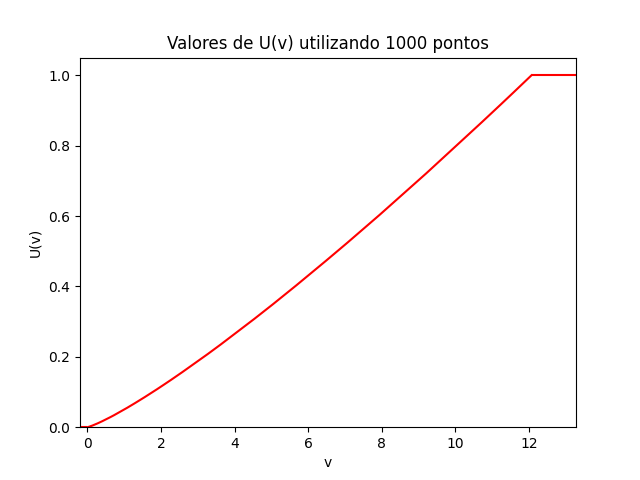
\includegraphics[width=0.5\textwidth]{Acumulada.png}
  \caption{Gráfico em x = [1,2,3] e y = [1,2,3]}
  \label{fig:HxU}
\end{figure}

Assim, conseguimos estimar a área de um gráfico que possui uma distribuição não-uniformemente randômica com a precisão desejada e vimos as formas de como conseguirmos obter a probabilidade total por meios computacionais.

\end{document}
